\section{Sovereign Cloud Stack}
\label{sec:gaia-x-einbettung:scs}

\begin{figure}[h]
  \centering
  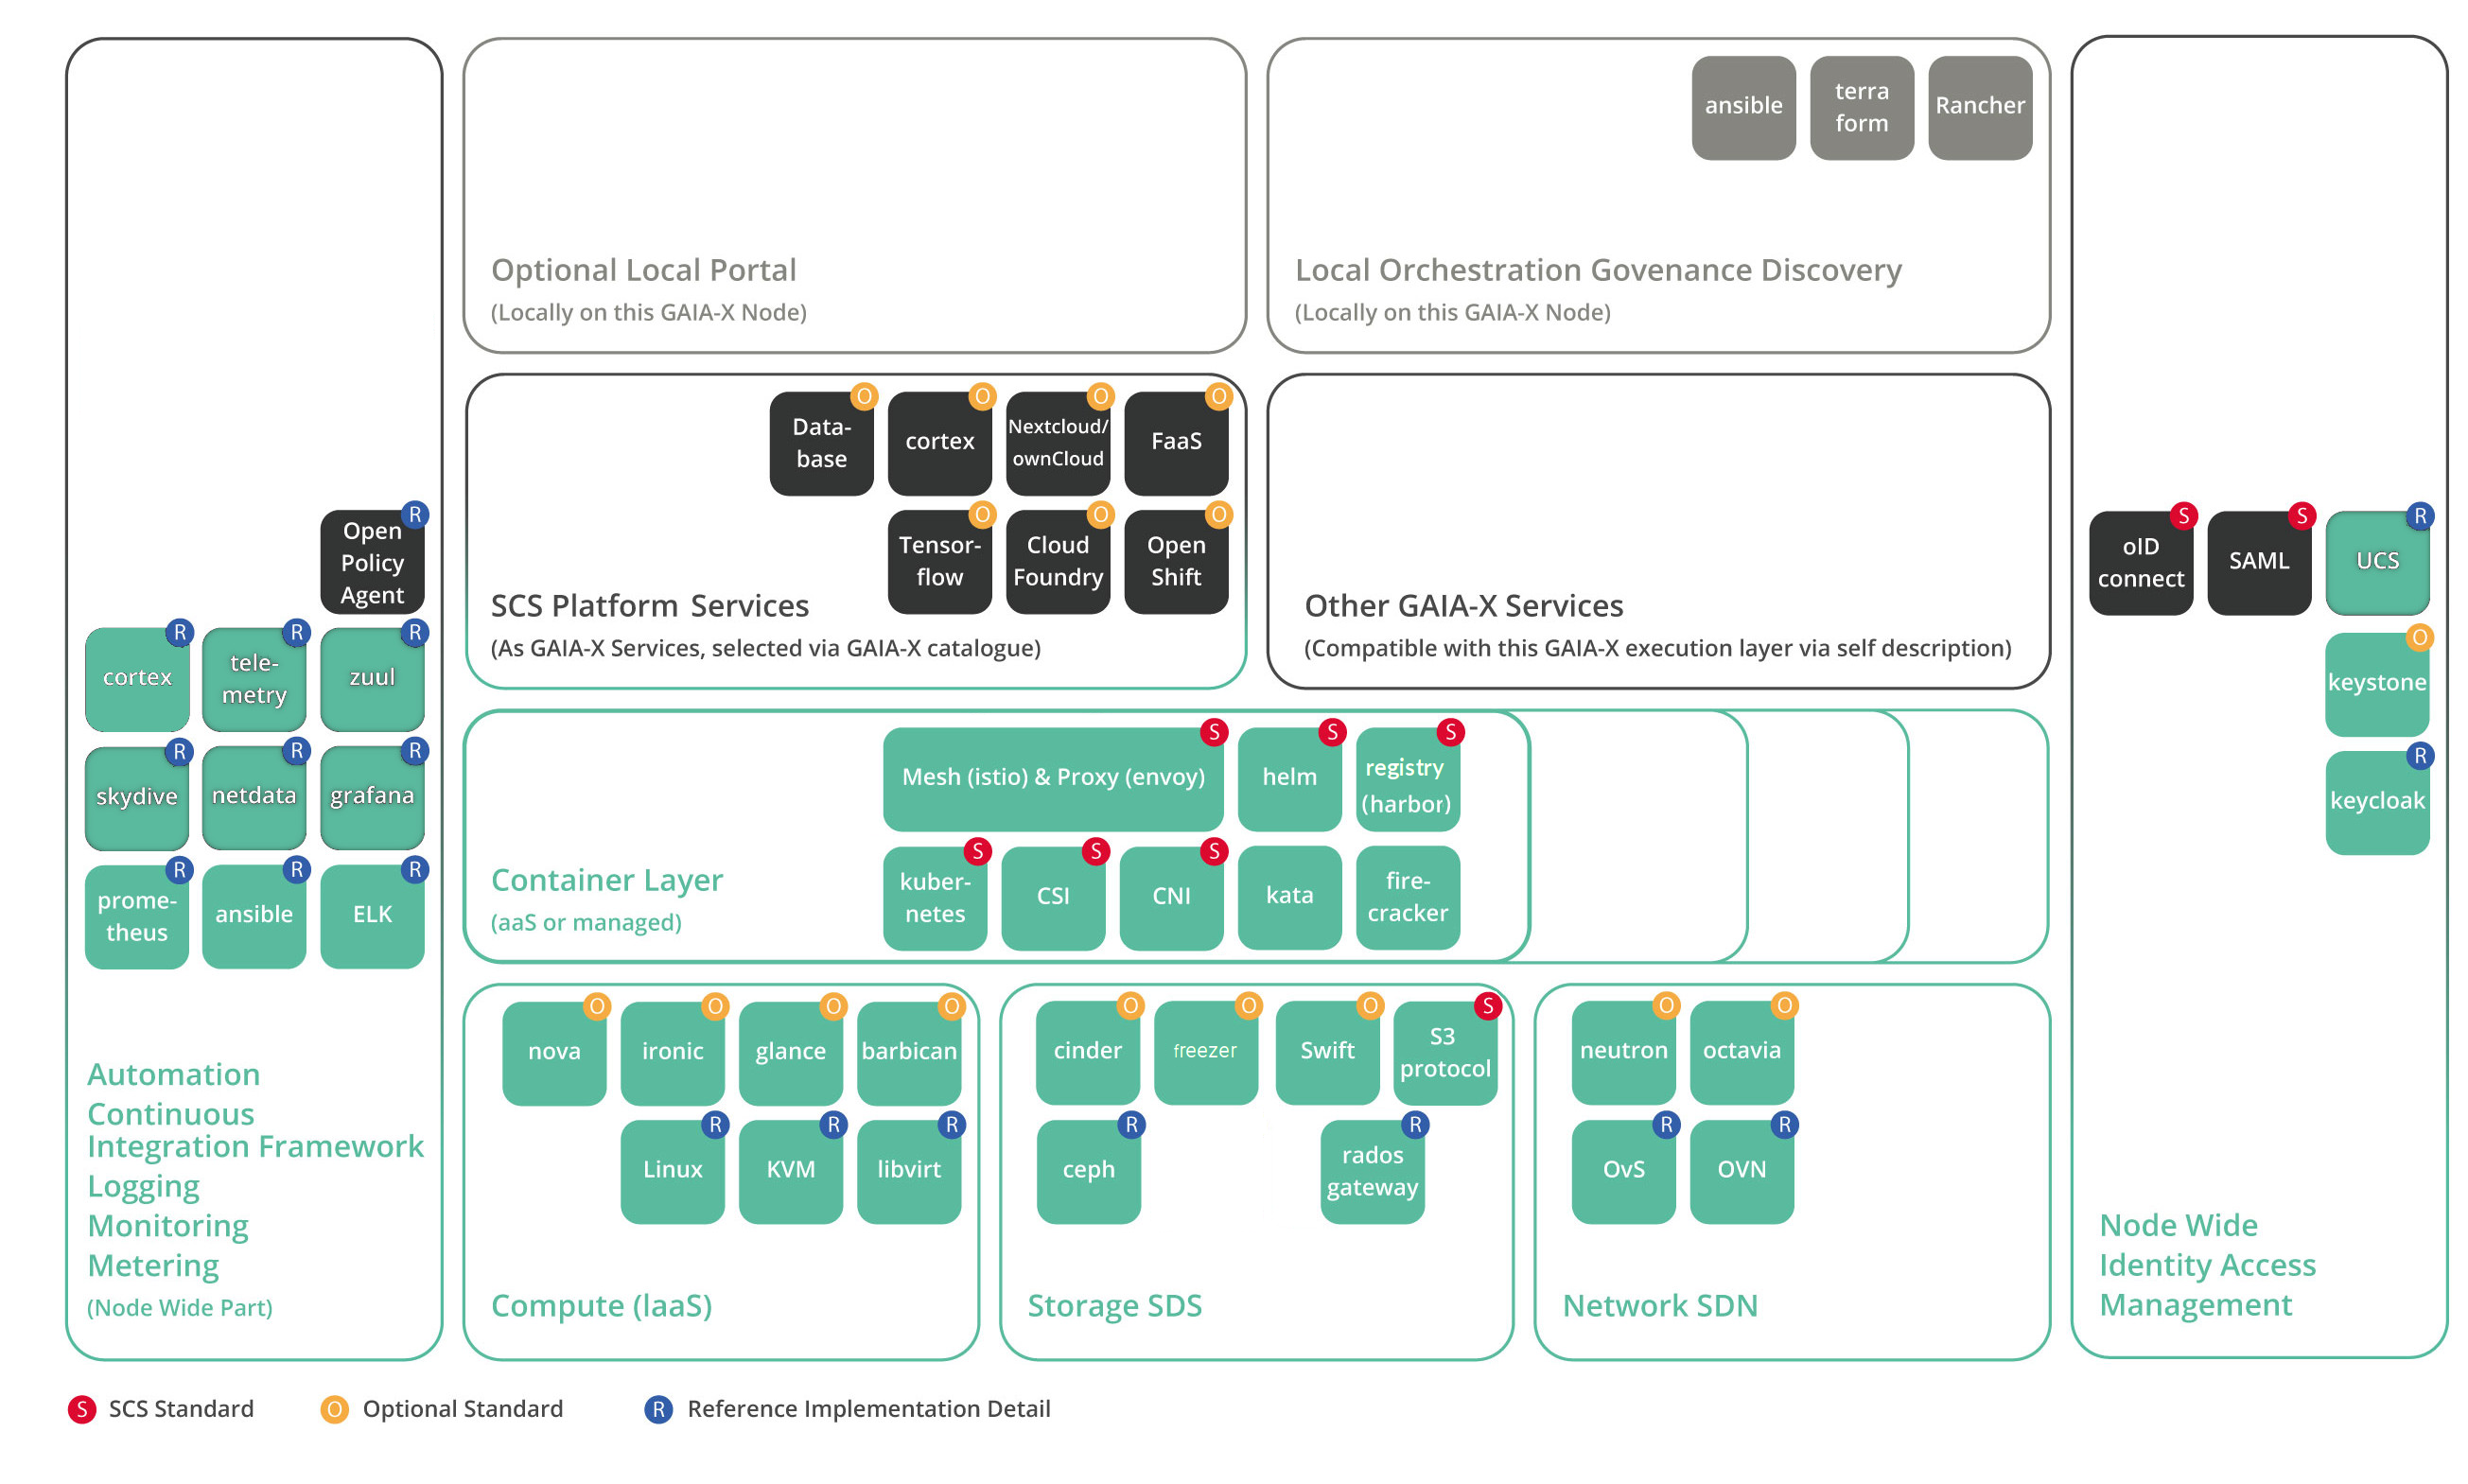
\includegraphics[height=0.71\textwidth]{gfx/chapters/4_gaia-X/scs_architecture.png}
  \caption{Architektur und Komponenten des Sovereign Cloud Stacks}
  \source{https://scs.community/assets/images/201001-SCS-4a.png}
  \label{fig:scs_architecture}
\end{figure}

\ac{SCS} ist ein Open-Source Projekt, um eine standartisierte und souveräne Plattform zu definieren, welche von 
existierenden und zukünfitgen Cloudprovidern genutzt werden soll. 
Ziel des Stacks ist ein Netzwerk von Anbietern, welche durch Nutzung von freier Software und gemeinsamer Standards,
eine interoperable, unabhängige Cloud schaffen.\cite{Kagermann2021}
Als technologischer Standpunkt dient \ref{fig:scs_architecture}, welches die geplante Architektur des \ac{SCS} zeigt. 
Grundlage des Stacks sind OpenStack Services, welche als OpenSource Projekt für Cloud-Computing Architektur entwickelt wurde.
Unterteilt wird dies in 3 grundlegende Bausteine: \textbf{Compute}, \textbf{Network} und \textbf{Storage}. Darauf aufbauend
wird ein Container Layer erstellt, welcher mit Hilfe von Containerruntimes wie Docker oder Podman\footnote{\href{https://podman.io}{Podman}} gesteuert werden soll.\cite{scs}
Services wie der in dieser Thesis entwickelte Chat \ac{SaaS} finden sich auf der übergeordneten Ebene \textbf{SCS Platform Services} wieder.
Für die Entwicklung des Rocket Chat \ac{SaaS} wurde diese Architektur als Grundbild genutzt, indem 
genannte Technologien des Stacks in der Implementierung berücksichtigt wurden.